\chapter{Wave propagating in a bound medium}
The wave propagated in some  arbitrary direction with respect to the coordinate axes have been studied and investigated from the last chapter. Henceforth we will study the wave propagation in a bound medium.As earlier started, when we have a bound medium ,the freedom to choose a coordinate axis is not really there. Hence in a bound medium,the choice of coordinate axis is that which when chosen, will align along the axis and then the wave propagates in arbitrary direction with respect to the coordinate axis because the wave is now incident on the boundary from some arbitrary angle.\\


\section{PLANE WAVE AT MEDIA INTERFACE}


Instead of having a finite medium,we can divide the medium into two semi infinite media thereby producing what is called a media interface between the two semi infinite media.\\The medium at the left of the media interface is infinite while that at the right of the media interface is infinite.Assuming on the left side we have medium 1 and on the right side we have medium 2 and also assuming that the conductivity$(\sigma)$ for both of the medium is still zero,that is the media  is still lossless but  the permitivity $(\varepsilon)$ and permeability($\mu$) for both media are different.\\Therefore


permeability for medium 1 =$\mu_1$ 

permeability for medium 2 $=\mu_2$

permitivity for medium 1$=\varepsilon_1$

permitivity for medium 2 $=\varepsilon_2$\\

If the coordinate system  was oriented such that the media interface is in  the xy plane,the x axis is the vertical axis , the z axis is the perpendicular axis that is  the axis perpendicular to the x axis ( 90$^{0}$ to x axis) and the y axis is pointing outward.This is shown in the  figure 1.
\begin{figure}
\centering
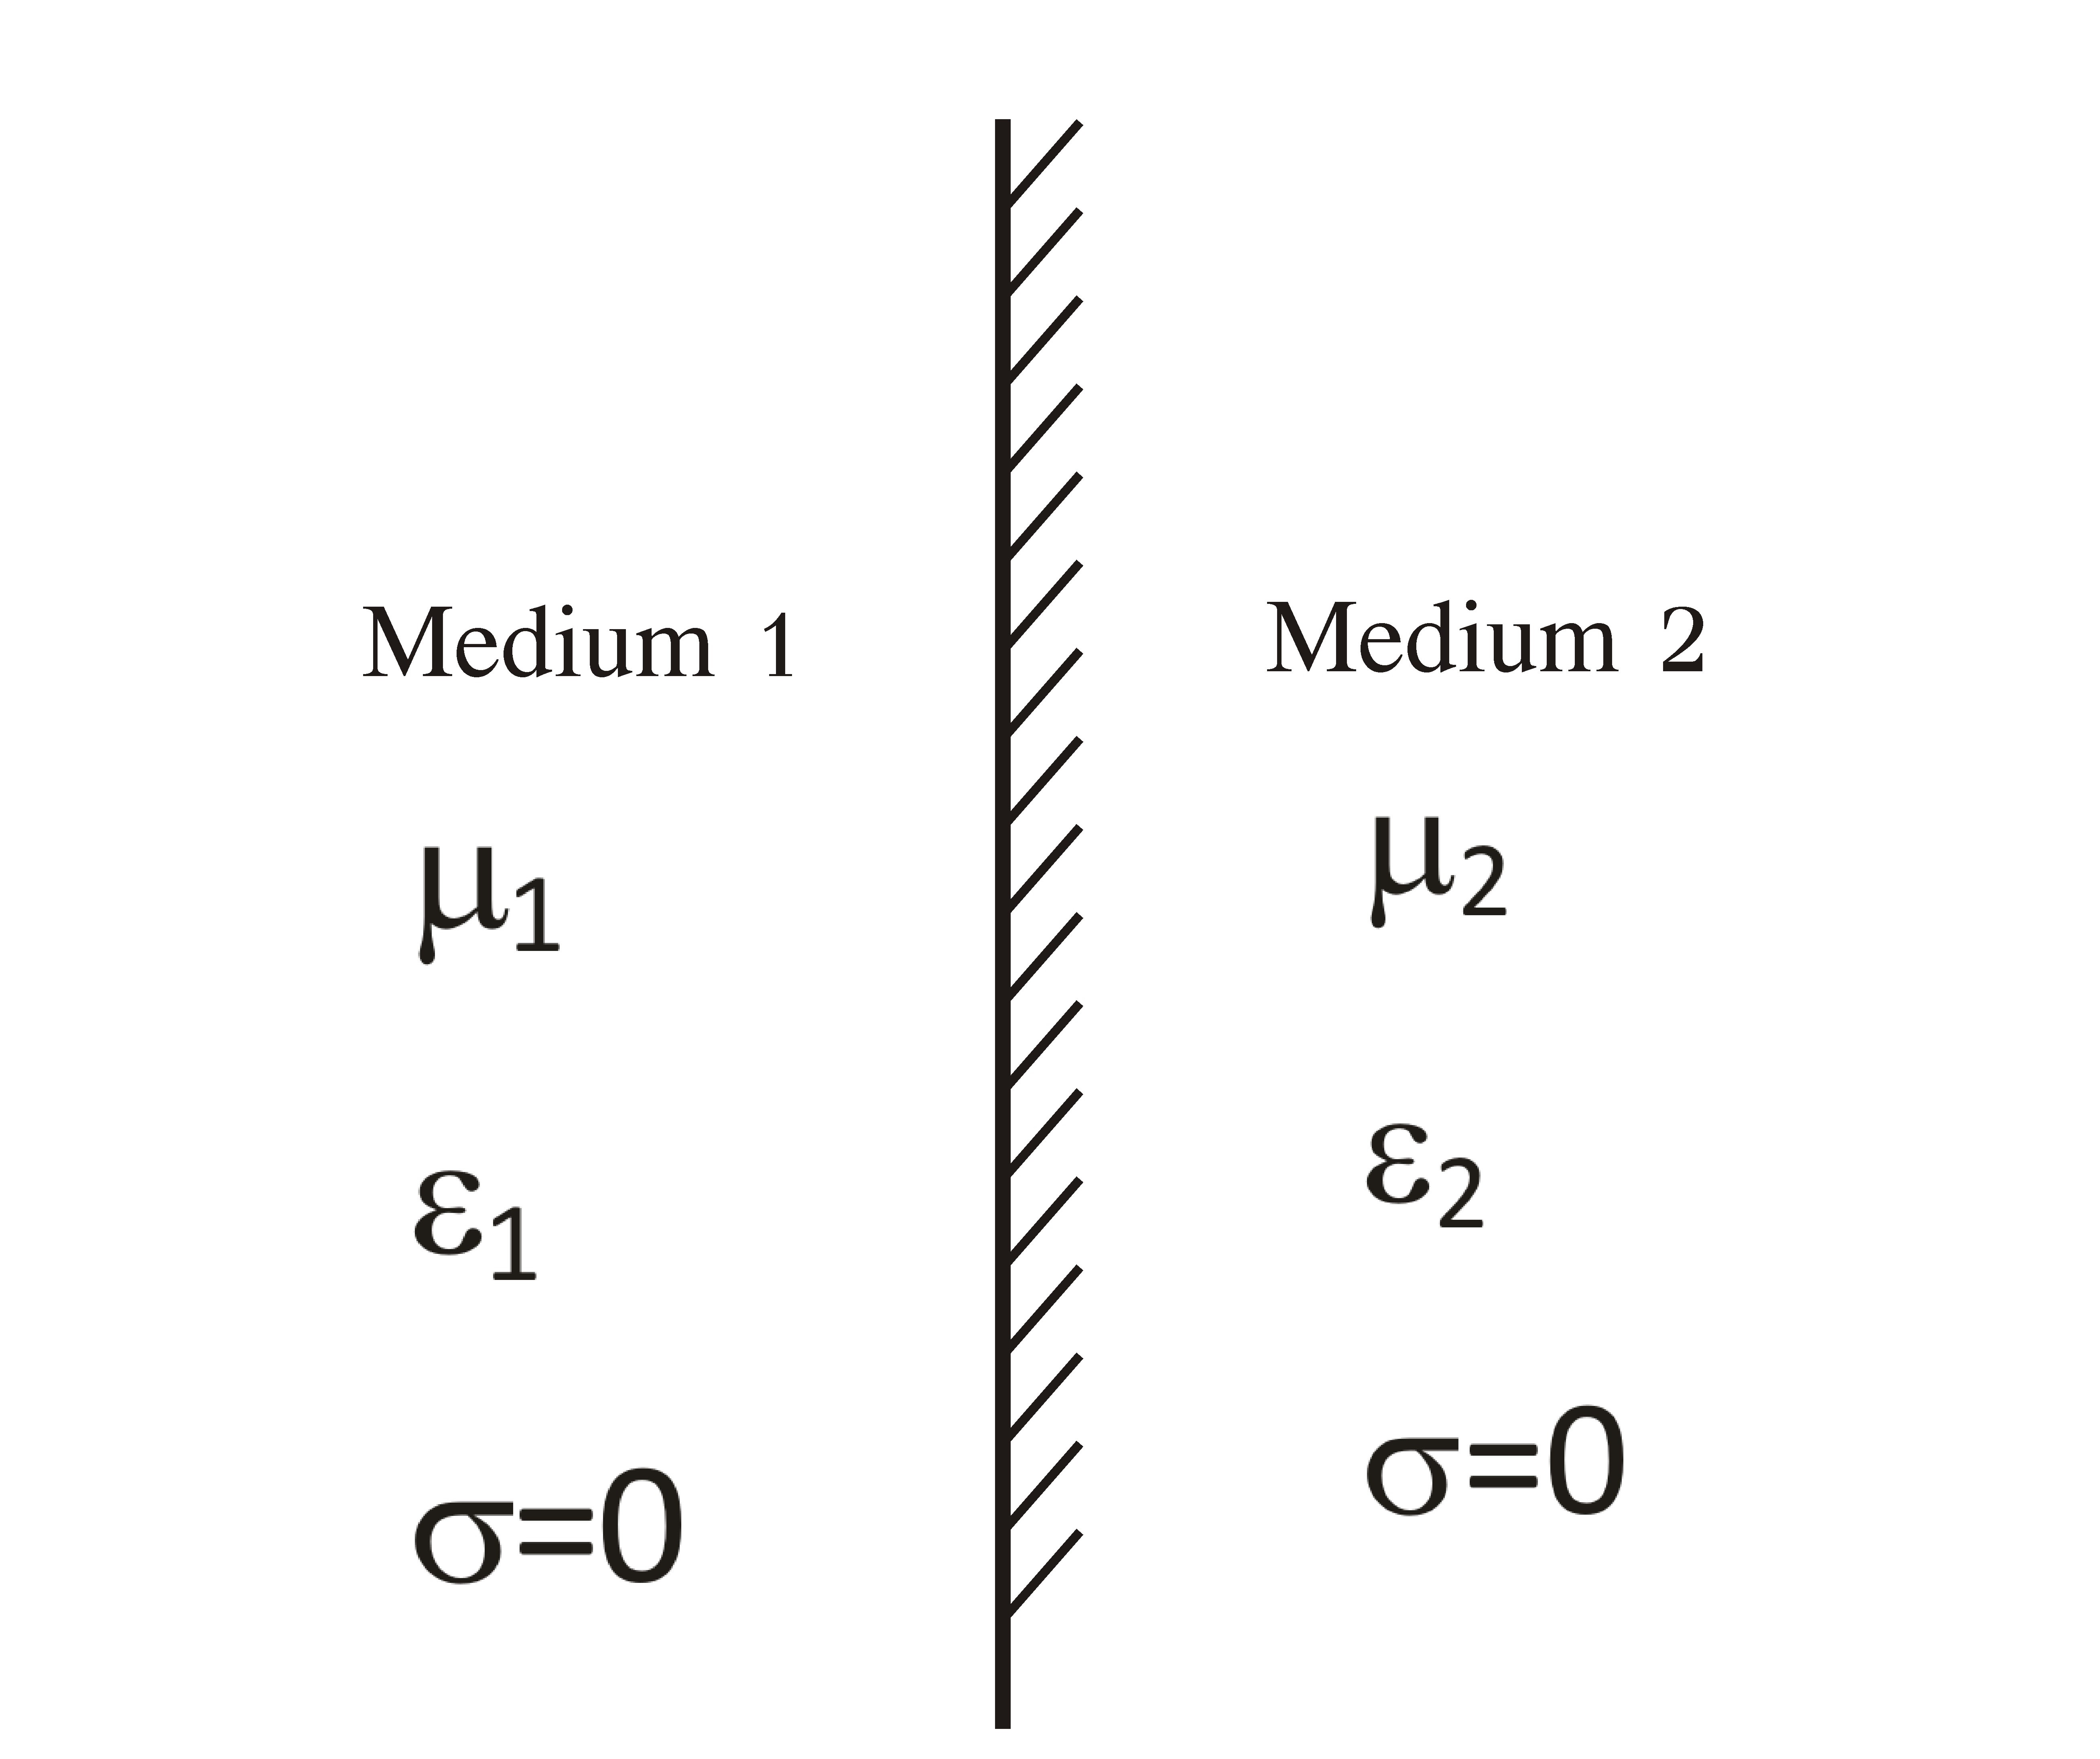
\includegraphics[width=.5\linewidth]{group30a}
\caption{}
\label{fig:group30a}
\end{figure}


\section{INCIDENT WAVE AT A MEDIA INTERFACE.}Given  a wave which is incident on the xy plane at some arbitrary angle with respect to the coordinate axis as illustrated in Fig 2.We may be wondering that when the wave is incident on the surface,what will happen to this wave?Some part of the energy of the wave will be transferred to the other medium (medium 2) which constitute some kind of wave propagation in medium 2.A phenomenon that is  not observed is that some part of the wave will get reflected  from the boundary interface back to medium 1.


So if the wave is incident on the media interface,part of the waves energy is transmitted to the second medium and continues with its propagation in medium 2.When the wave is incident on the media interface,two kinds of field will exist.One will be existing in medium 2 and also the field in the first medium must be modified to satisfy the boundary conditions.Part of the energy goes into the second medium and part of the energy gets reflected, that is comes back to medium 1.\\

As a result of this, what happens to the plane wave nature?In what direction will the energy be going?what is the magnitude of the field going into the second medium and how much power is transfered into the second medium?How much power gets back from interface to the first medium and what happens to the direction of electric field.These are some of the issues that relates to propagation of uniform plane waves at media interface.The media interface becomes a dielectric interface if conductivity is zero as in this case.\\ let $\theta_i$ be the angle of incidence at the media interface (the angle between the plane wave and the normal to the xy plane)as shown in fig 3 above.the media is uniform in the xy direction and the sudden change in uniformity is at z=0.The z direction as we have seen is perpendicular to the media interface and hence it is the normal to the media interface.So what happens to the wave when it is incident to the media interface at this angle $\theta_i$.The wave is first represented in a form which is a phase and amplitude without specifically saying whether we are referring to electric or a magnetic field.So the wave has some field vectors with the definite phase function since it is traveling at an angle $\theta_i$ with respect to the coordinate axis.	

Hence this vector makes three angles $\theta_x$,$\theta_y$,$\theta_z$.$\theta_x$ is the angle which the wave makes with the x axis and it is =($\pi\div2$)-$\theta_i$.The angle $\theta_y$is the angle it makes with the y axis which is ($\pi\div2$) and $\theta_z$=$\theta_i$.With these angles known, the direction cosines can  written down  and then   the phase function can be written down.Let $\beta_1$ and $\beta_2$ be the phase for medium 1 and medium 2 respectively.

$\beta_1=\sqrt{\mu_1\varepsilon_1}$.

$\beta_2=\sqrt{\mu_2\varepsilon_2}$.\\
let $\bar{F_i}$ represent this wave incident on the interface(it can be electric or magnetic field)with magnitude$\bar{F_{oi}}$,then\\ $\bar{F_{i}}=\bar{F_{oi}}exp^-j\beta_1{\cos\theta_xx +\cos\theta_yy+\cos\theta_zz}$.Since \\$\theta_x=(\pi\div2)$-$\theta_i$,\\$\cos\theta _x=\sin \theta_i$.\\$\cos \theta_y$=0,\\$\cos\theta_z=\cos \theta_i$.\\Substituting in the incident wave vector,\\$\bar{F_i}=\bar{F{oi}}\exp -j\beta_1(\cos \theta_x+\cos \theta_y+\cos \theta_z)$.\\So the wave  which is traveling at an angle $\theta_i$ with respect to the normal to the interface can be represented by a field\\ $\bar{F_i}=\bar{F{oi }\exp j\beta_1(x\sin \theta_i+z\cos \theta_i)}$.\\At some instant of time,the variation of the field amplitude as a function of x,y and z is obtained by taking the real part of $\bar{F_i}$
\\ magnitude of field on the xy plane at z=0 =Re($\bar{F_i})$=$\bar{F_{oi}}\cos (\beta_1x\sin \theta_i)$
\begin{figure}
\centering
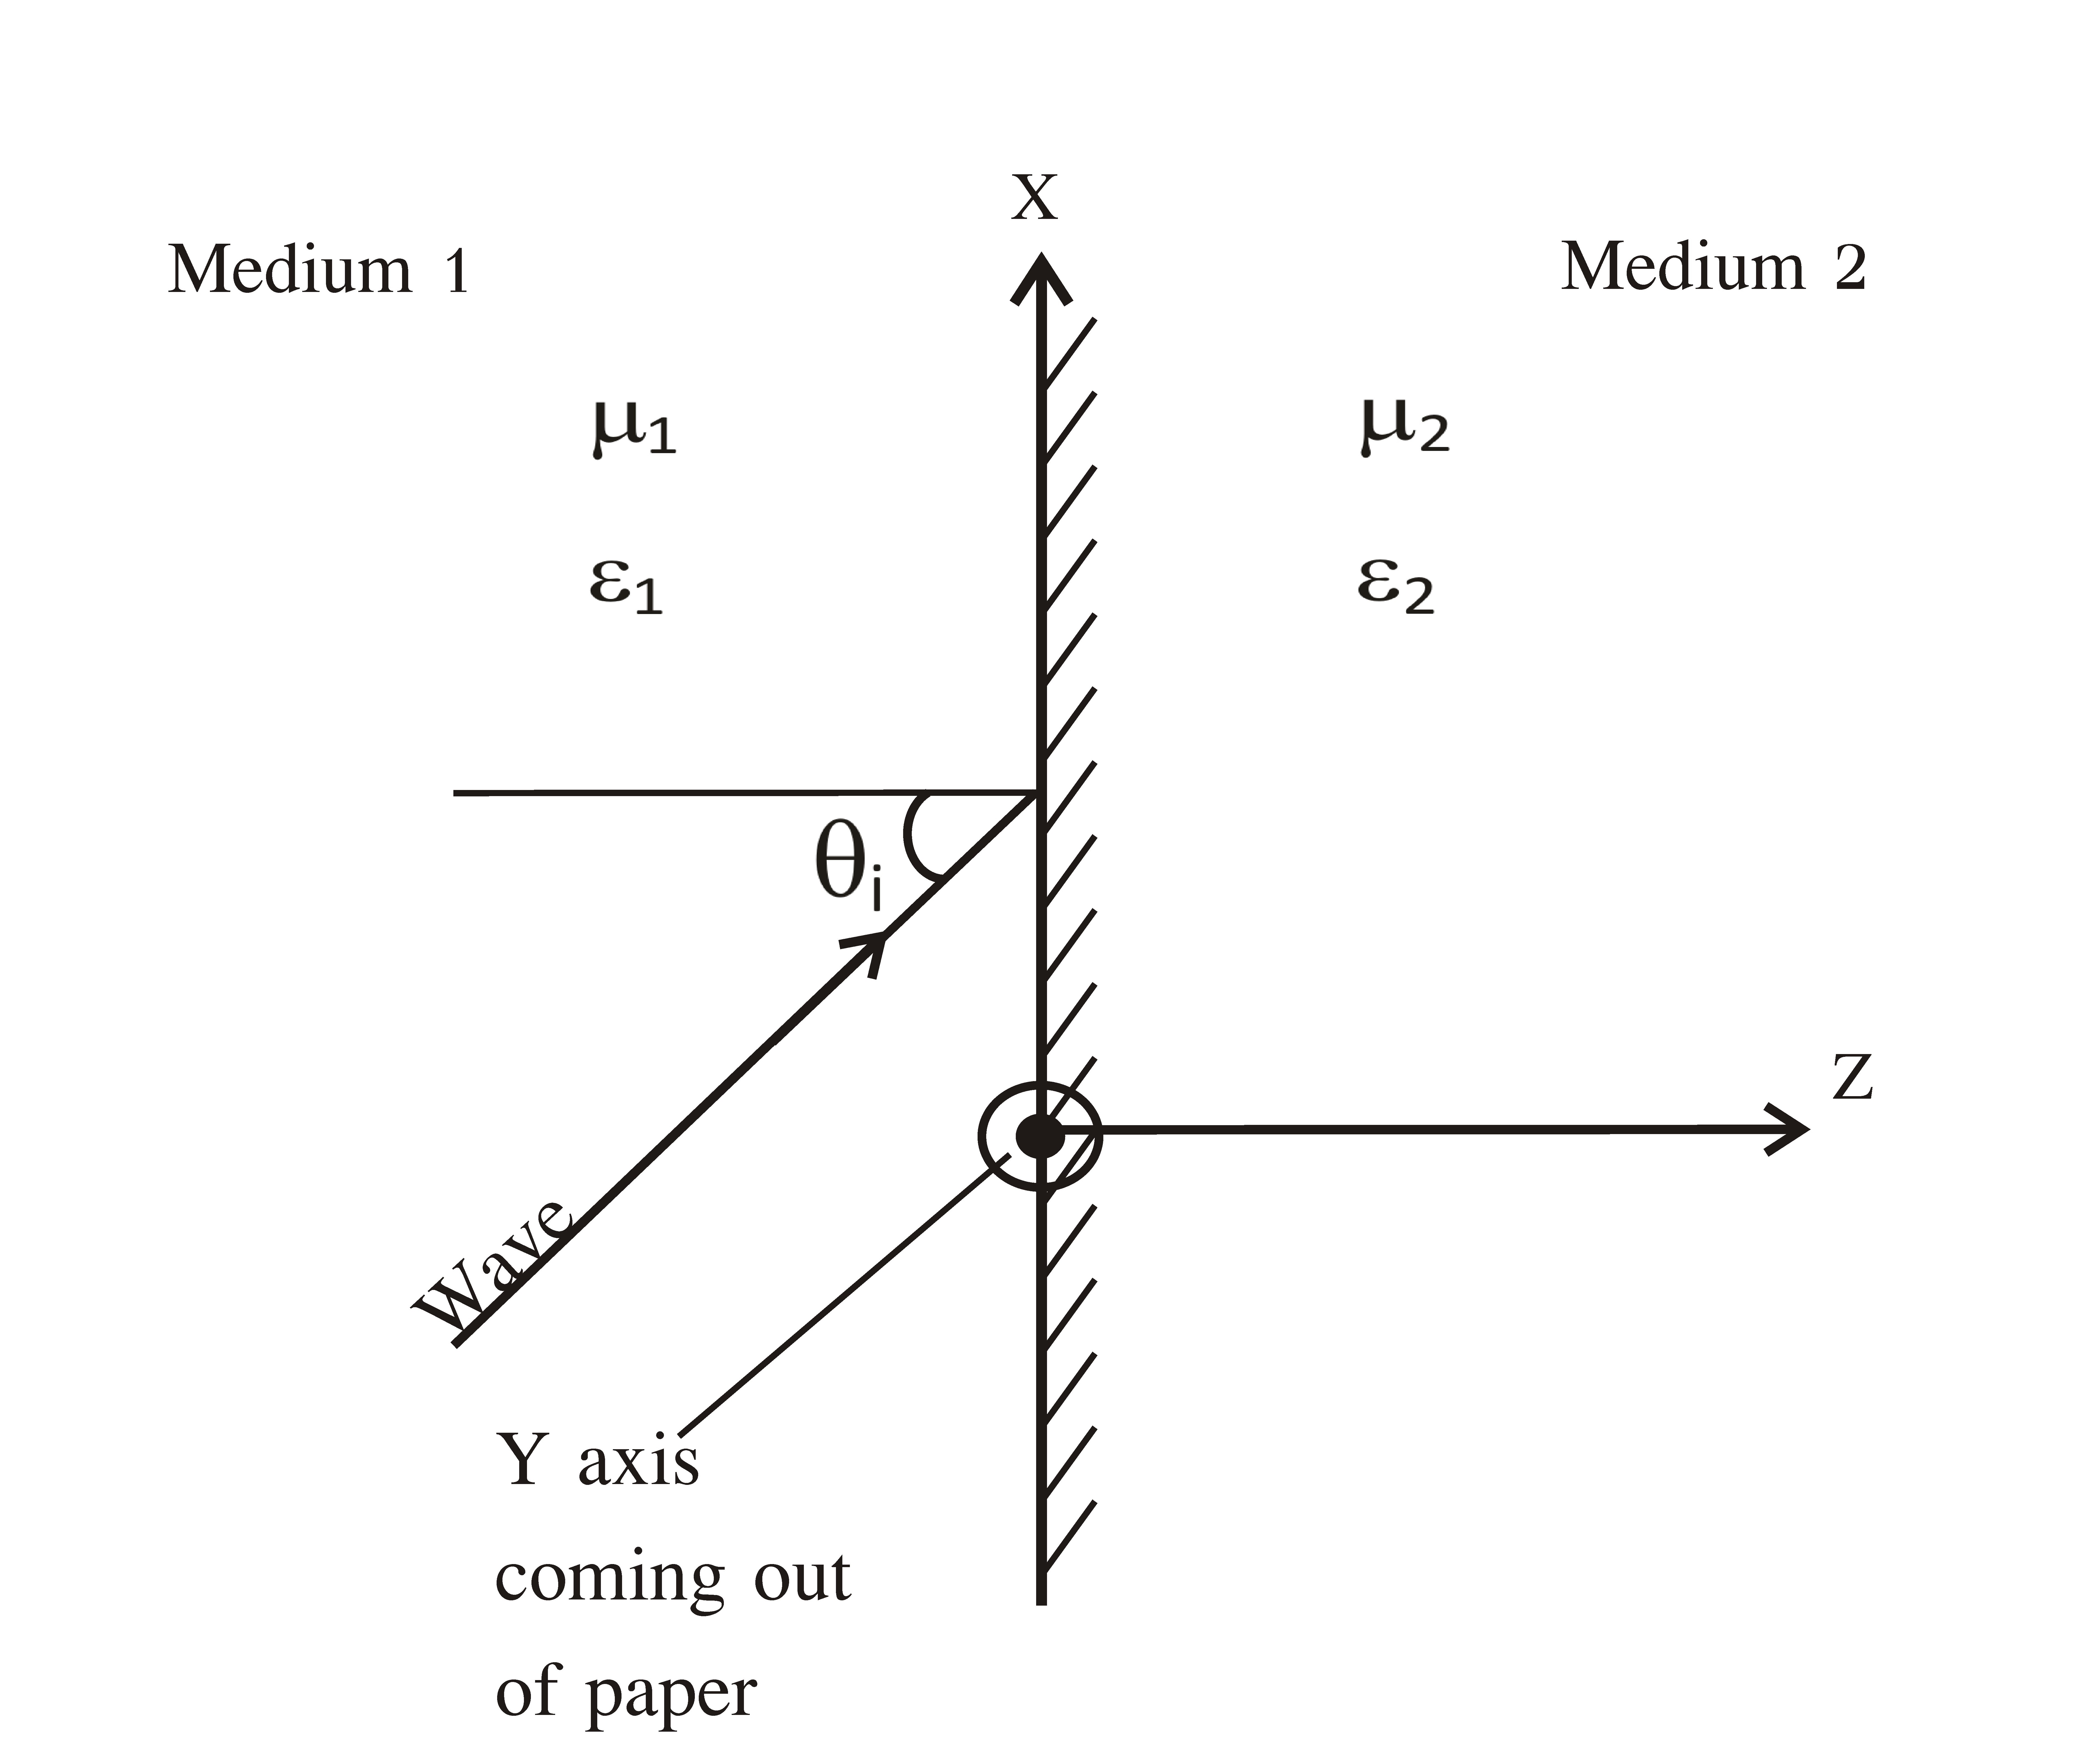
\includegraphics[height=5cm]{group30b}
\caption{}
\label{fig:group30b}
\end{figure}


So the field is having a variation which is cosine variation in the x direction and it does not have any variation in the Y direction. If the field were to be plotted,the amplitude will vary along the X axis and it will be constant on the y direction as shown below.

\begin{figure}
\centering
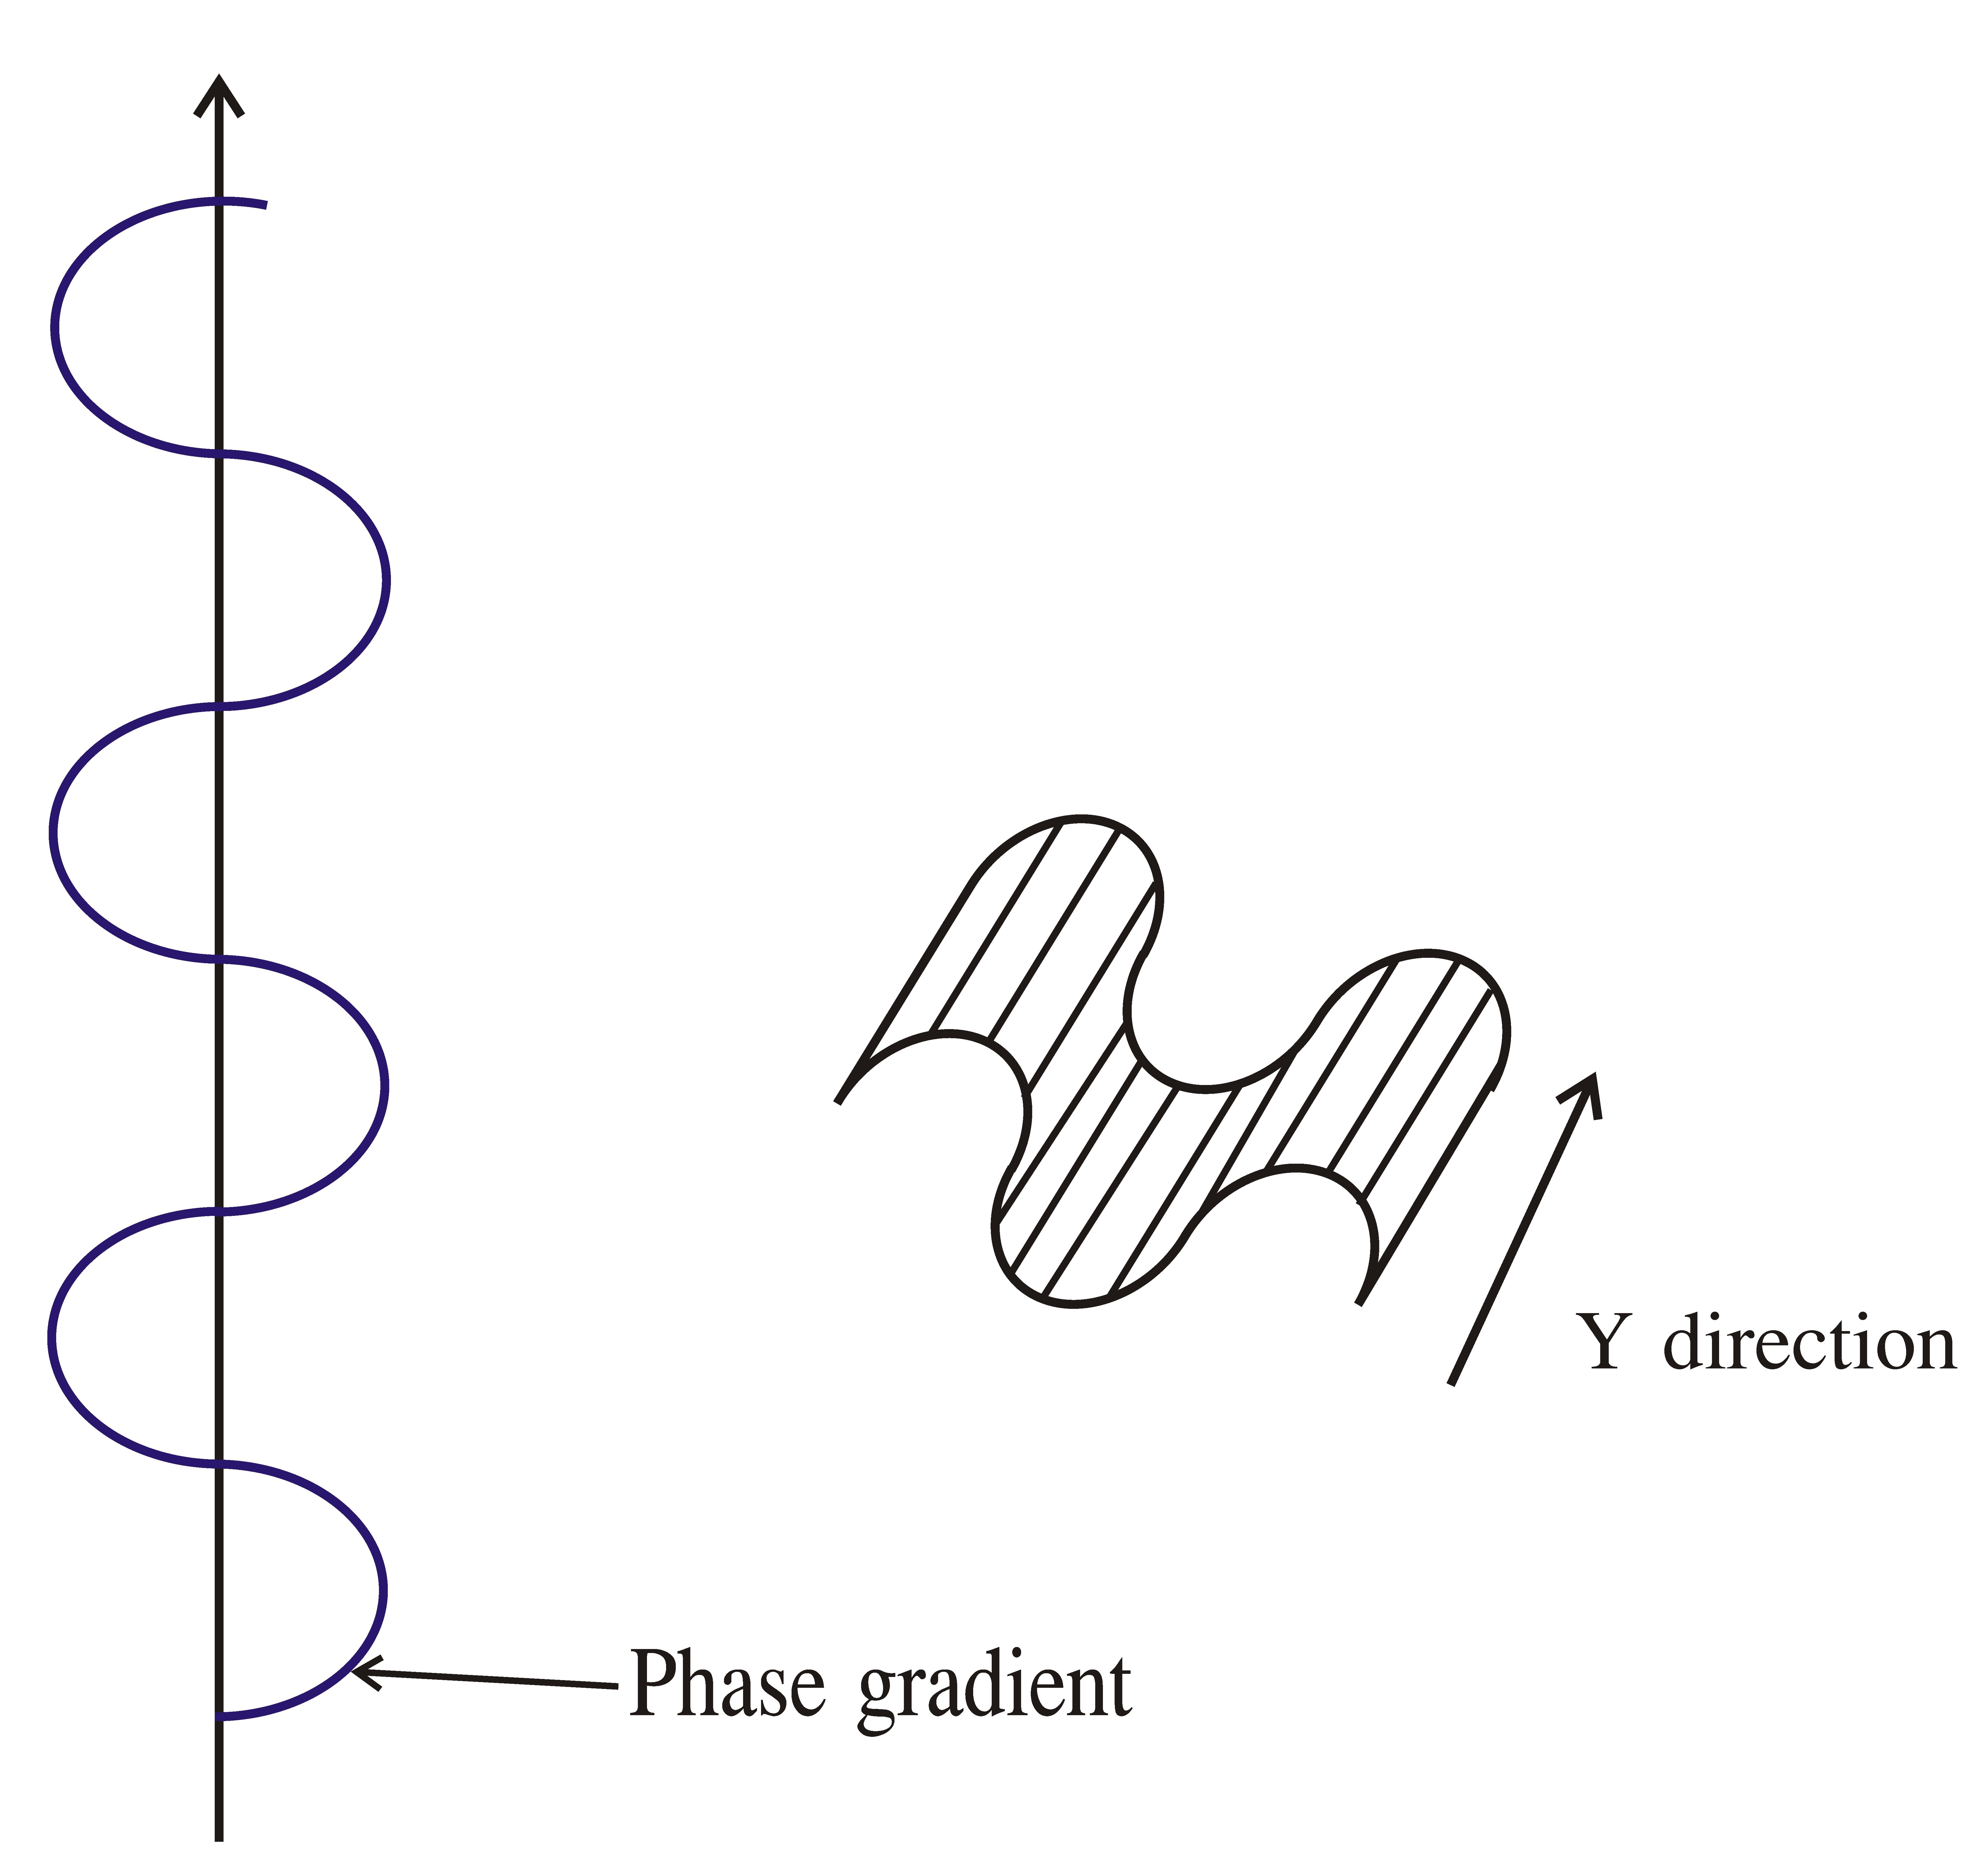
\includegraphics[height=5cm]{group30c}
\caption{}
\label{fig:group30c}
\end{figure}

Essentially it is more like a corrugated surface on the xy plane(think of a zinc sheet for roofing).it has the abestos sheet planon of undulation as shown below in figure above.

it has been established that if  the wave is incident in the direction shown,the amplitude variation on the xy media interface appears like a corrugated surface.So we can visualize the field as an amplitude variation in the x direction or it has a phase variation $\beta_1\sin \theta_i$ or phase gradient -$\beta_1\sin\theta_i$ .The phase gradient will be equal to zero if $\theta_i=0$.\\Thus, the phase becomes constant and this is what happens when the wave is moving perpendicular to the xy plane and therefore will not have any gradient in that plane.So the direction of the wave as it changes affects the phase gradient in the plane.

Creating a phase gradient and changing  the direction of the wave is similar.This simply means that changing the wave direction leads to a particular gradient and also creating a phase gradient leads to a wave that orient in the same direction to satisfy the phase gradient.If the phase gradient at the interface is given and this value of  phase gradient is equated to to $-\beta_1 \sin \theta_i$,we get some quantity $\theta_1$ and this gives us the effective direction in which the wave is traveling.In essence,this simply means that  if a wave is given in some arbitrary direction,a phase gradient in created but if the phase gradient is given,we get a wave traveling at an angle that will satisfy the phase gradient created.

we have seen the wave traveling from medium 1  which was making an angle $\theta_i$ with respect to the media interface and has also seen that the wave creates a phase gradient.If the wave was incident from medium 2 in the direction of $\theta_i$,it creates exactly same phase gradient on the xy plane.So irrespective of whether this incident wave is coming from medium 1 or 2 both are going to creates exactly same phase gradient on the media interface.


\begin{figure}
\centering
\includegraphics[height=5cm]{group30d}
\caption{}
\label{fig:group30d---copy}
\end{figure}

From the diagram in figure 4 above,waves A anb B are incident wave from medium 1 and medium 2 respectively.These two waves will create the same phase gradient respectively.B in medium 2 corresponds to a wave B'  at an angle $\theta_B$ traveling away from the interface in medium 1.A in medium 1 corresponds to a wave A' at an angle $\theta_A$ traveling away from the interface in medium 2 .

A wave which is approaching the interface and a wave which is going away from the interface at the same angle made with respect to the normal creates the same phase gradient.Two other waves and their direction that can result to same phase gradient are B'
and A.B' is a result of reflection of incident wave A and A'is a result of the wave transmitted into the medium 2 as a result of incident wave A.All these waves result in a constant phase gradient at xy plane when z=0(A' is called the transmitted wave or refracted wave and B'is called the reflected wave and wave A that brought energy to the media interface is called the incident wave as shown in figure 4 above.



In general, the wave vector for incident wave ,reflected wave and transmitted wave all lie on the same plane called the plane of incidence.The y axis is perpendicular to the plane of incidence.the important conclusion is that when a wave was incident on a dielectric interface(in this case) at an angle, it induces two waves called the reflected wave going from the interface through medium 1  and  the refracted  wave going away from the interface to medium 2 as illustrated in figure 4 above.
.All these three waves have the same phase variation and all lie in the same plane called the plane of incidence.If E is the magnitude of electric field and H is magnitude of magnetic field,then(E$\div$H)=$\eta$ holds for medium 1 and medium 2 as the wave always sees an infinite medium ahead of it media interface.This incident wave always excite electric and magnetic field in medium 2.this excitation creates E and H that will satisfy (E$\div$H)=$\eta_2$.$\eta$ is known as the intrinsic impedence.it is clear that we cant satisfy boundary conditions by having E$\div$H=$\eta_1$ in  medium 1 and E$\div$H=$\eta_2$ In Medium 2 for both electric and magnetic field.This means that a certain field has to be induced in the first medium.In other words we have to modify the fields in the first medium so that the boundary condition can be satisfied for electric and magnetic fields at the interface.so there will be fields induced in both medium 1 and medium 2 due to the incident wave in order to satisfy boundary conditions.The reason is that the incident wave leads to both refracted wave in medium 2 and reflected wave in medium 1 as shown in figure 5 below.since the inducing phenomenon is due to phase variation,the two other waves induced in the interface will have same phase variation as the original incident wave.since the fields are time varying,they constitute a wave phenomena.

\begin{figure}
\centering
\includegraphics[height=5cm]{group30e}
\caption{}
\label{fig:group30e}
\end{figure}


We recall that light is a transverse electromagnetic wave and if we can recall the various laws of reflection for light,the first law states that the incident ray,reflected ray and transmitted ray all lie on the same plane called the plane of incidence.so the first law of reflection comes from satisfying the phase condition on the interface.the plane of incidence is that which  contains the wave vector and the normal to the interface,.thus we get the first law of reflection established by the phase condition.

if -$\beta_1\sin \theta_1$ is the phase gradient created because the wave moved in medium 1,for medium 2,$ 
\theta_2$ is obtained by equating the phase gradient in medium 1 and medium 2(that is -$\beta_1\sin \theta_1=-\beta_2\sin \theta_T,where \theta_T$ is the angle the transmitted wave makes with the normal.) .In general the angle which the waves makes with the normal is given by the formula below

$\theta=(phase gradient\div phase constant)$.

let $\theta_r$ and $\theta_t$ donate the angle of reflection and the angle of refraction respectively.The diagram below clearly explain$\theta_r$ and $\theta_t$.from\\  $-\beta_1\sin \theta_i$=$-\beta_1\sin \theta_r$\\ 

$\sin \theta_r$=(-($-\beta_1\sin \theta_1) \div(\beta_1$).\\From the above formula we get\\ $\theta_i=\theta_r$.\\This is called the second law of reflection that is the angle of incidence and the angle of refraction are equal.This law is a familiar law in optics that if a light ray is incident on an angle and the refractive index of the two medium are given as $m_1$ and $m_2$ respectively,then the transmitted or reflected angle $\theta_T$  is given by 
\\ $\sin \theta_T=(m_1\sin\theta_i)\div(m_2)$.\\This is a special case of snells law.

So whatever angle of incidence with respect to the normal it is the same angle with which the wave is reflected.
similarly\\-$\beta_1\sin\theta_1=-\beta_2\sin\theta_2$. (phase gradient must be the same to have the same phase variation)or\\ $\sin\theta_i\div\sin\theta_T$=$\beta_2\div\beta_1$.But $\beta_1=\omega\sqrt{\mu_1\varepsilon_1}$ and also $\beta_2=\omega\sqrt{\mu_2\varepsilon_2}\sin\theta_2$ substituting,we have\\ $\omega\sqrt{\mu_1\varepsilon_1}\sin \theta_1=\omega\sqrt{\mu_2\varepsilon_2}\sin\theta_2$.$\omega$ cancel and the resulting equation gives the Snell's law.This is the important law which tells the direction of transmitted electromagnetic waves with respect to the direction of incident waves.we call this the generalized Snell's law.So for pure dielectric with $\mu$ negligible,Snell's law reduce\\ $\sqrt{\varepsilon_1}\sin\theta_1=\sqrt{\varepsilon_2}\sin\theta_2$.\\If $\varepsilon_{r1}$ and$ \varepsilon_{r2}$ is the refractive index of medium 1 and medium 2 respectively and $\varepsilon_{r1}=n_1$ and $\varepsilon_{r2}=n_2$,then\\ $\sqrt{\varepsilon_o\varepsilon_{r1\varepsilon}\sin\theta_i}$=$\sqrt{\varepsilon_o\varepsilon_{r2}\sin\theta_2}$ reduces to $n_1\sin\theta_i=n_2\sin\theta_T$.

Therefore in summary we started the wave propagation in some arbitrary direction .in this arbitrary direction,it creates a phase gradient in the media interface.This phase gradient is the same for the wave which are induced in both sides of the media called transmitted wave and reflected wave.We found that changing the direction of the wave and changing the phase gradient are essentially equivalent.Hence the induced field have the same gradient in the interface and there essentially we can find out the direction in which the wave will be traveling.from these the laws of reflection and Snell's law were established.Lets consider the diagram figure 6 below
where we have the magnitude of  the electric field .the arrows shows the wave direction of  propagation meaning that the electric field is oriented in some other direction.So with amplitude,$\bar{E}$,$\bar{E_r}$,and $\bar{E_T}$ ,We want to find out the relationship between $\bar{E_t}$ and $\bar{E_i}$ which is( $\bar{E_t}\div\bar{E_i}$ ).
\begin{figure}
\centering
\includegraphics[height=5cm]{group30f}
\caption{}
\label{fig:group30f}
\end{figure}

This quantity is what we call the TRANSMISSION COEFFICIENT the ratio 0F the interface.The ratio of$ E_r$ to$E_i$ is what we call the reflection coefficient.We have some situation that when the wave sees a a change in intrinsic impedance which causes impedance discontinuity,a part of the energy is reflected and   the reflection coefficient is $\bar{E_r}\div\bar{E_i}$.The reflection coefficient $\Gamma=(\bar{E_r} \div\bar{E_i}$) ,transmission coefficient $\tau$=($E_t$)$\div$($E_i$).So we have $\Gamma$and $\tau$ as electric field reflection coefficient and electric field transmission coefficient .These quantity can be define for magnetic fields also $\tau$.As already know,the $\bar{E}$and$\bar{ H}$ fields are related by the intrinsic impedance of the medium.if we know $\bar{E}$,$\bar{H}$ can be found out since( $\bar{E}$$\div$$\bar{H}$)=$\eta$ where $\eta$ is the intrinsic impedance.So for medium 1 $( \bar{E_r}\div\bar{H_r})=\eta_1$  and $(\bar{E_t}\div\bar{H_t})=\eta_1$.For medium 2,$(\bar{E_t}\div\bar{H_t})=\eta_2$ .$\eta_1$ and $\eta\eta_2$ are the intrinsic impedance for medium one and medium 2 respectively.The electric field will be in a direction  with  an angle to the plane of incidence in which the wave vector lies.This electric fields can be resolved into two components.These are parallel polarization where the electric field lie in the plane of incidence and perpendicular polarization in which the electric field lies perpendicular to the plane of incidence.$\Gamma$ and $\tau$ has to be calculated for in order to analyse these two cases.once this is done,the total characteristics of the wave which is polarized in an arbitrary angle can be examined.